\chapter{Instructions for officers}
This assumes you have super-user privileges.
So it contains some higher-level administration tasks.

\section{Uploading scans (the scanning squad)}
Self-explanatory in theory, but hard to in practice.
Usually, we end up having a squad of about five people
who sit next to a scanner and process all the incoming exams.
Here is my suggestion for how to do it:
\begin{itemize}
	\ii Pre-process the paper:
	\begin{itemize}
		\ii Remove staples from scans, if any.
		You should have a squad of people do this \emph{en masse}
		in the volunteer room, before sending them to the scanners.
		\ii At the moment we don't have image processing,
		so please \textbf{make sure all scans are correctly rotated and oriented}.
	\end{itemize}

	\ii \textbf{\color{red} Upload the scans in grayscale, NOT black/white or color}.
	Using color slows down processing, and using black/white makes the scan
	illegible since we generally print exams on colored paper.

	\ii I strongly recommend using the \textbf{following organizational procedure}:
	\begin{itemize}
		\ii Upload the scans in batches of 20 pages each.
		(Batches longer than this may cause issues on most scanners).
		\ii Number the batches $1$, $2$, \dots, $n$.
		Write the number of the batch in sharpie on the first page,
		and upload it with the number in its filename.
		\ii After scanning a batch, staple it and put it aside.
	\end{itemize}
	It seems better to create the batches before sending
	them to the scanners.

	It is worth double-checking batches have the right size
	(and that no pages are rotated).

	\ii For safety, uploaded filenames \emph{must} be distinct.
	(This is to prevent someone from accidentally submitting the form twice,
	or submitting the same PDF twice.)
	Filenames must end with either ``pdf'' or ``PDF''.

	\ii \emph{Please}, make sure you are uploading the scans
	to the correct contest!
	There are some ways to deal with such mistakes but better
	if they can be avoided in the first place.
\end{itemize}

\begin{center}
	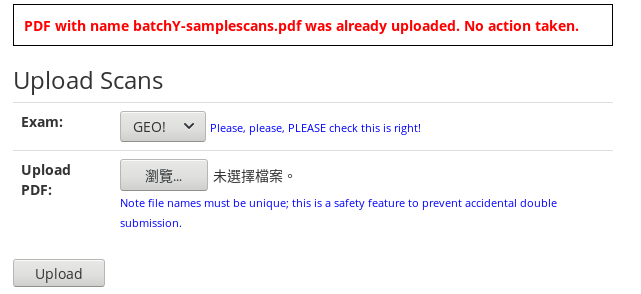
\includegraphics[width=0.8\textwidth]{images/batchscan.png}
\end{center}

When you upload a scan,
several problem scribbles, exam scribbles, and verdicts
are immediately created corresponding to the items in the PDF file.
However since the system does not yet know who is who,
the verdicts and problem scribbles will not have an entity attached to them.
The ``match scans'' functionality will then pair them up.

It seems preferable to upload scans in smaller batches,
rather than all at once.
This way, after the first PDF is uploaded,
graders can start marking immediately
while future PDF's are uploaded.

\section{Marking exams as ready}
In the Django administration interface,
there are two switches you need to flip for every exam:
\begin{itemize}
	\ii You can mark an exam as ``ready to grade'',
	meaning that its names can be matched and its answers graded.
	\ii Separately, you can enable the uploading of scans
	(``can upload scans'').
\end{itemize}
These are safety features designed to minimize the risk
of someone accidentally uploading scans to the wrong test, for example.

\section{Conflict resolution}
First, I should describe the logic behind verdicts.
For each exam there are two parameters:
\begin{itemize}
	\ii A \textbf{minimum majority} for the verdict to be valid,
	defined as a constant $n$ such that an $n$-to-$1$ majority suffices.
	The default is $n=4$.
	\ii If valid, a \textbf{minimum number of graders} needed before
	the verdict considers itself done.
	(So setting this number to $2$ is double-grading,
	$3$ is triple-grading, $4$ is quadruple-grading, \dots.)
	The default is triple-grading.
\end{itemize}

Officers get an extra panel called ``View All Conflicts''.
This lets you see the grading conflicts for \emph{everyone}.

\begin{center}
	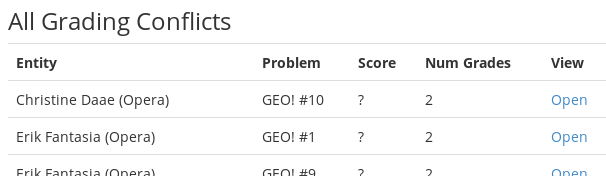
\includegraphics[width=0.8\textwidth]{images/all-conflict.png}
\end{center}

Given a conflict, you can open the verdict page corresponding to it,
at which point you can submit your own evidence.
If you like being final authority,
there should also be an option to submit this evidence in ``God mode''
which will settle the verdict once and for all.

Starting in 2018, Helium will actually stop giving sufficiently
controversial answers out for grading
(specifically, it will not give a problem out during normal grading
if more than $2n+2$ people have read it already).
So this is necessary to deal with those super-controversial answers.

\section{Find papers}
You can locate specific papers
by selecting ``Find Papers'' from the index page.
Some ways to do so:
\begin{itemize}
	\ii You can look up by exam and entity.
	\ii You can scroll through the pages of the PDF files.
	\ii A list of papers which need moderator attention
	will appear here (see Section~\ref{sec:view_full}).
	Dealing with them described in next section.
\end{itemize}

\begin{center}
	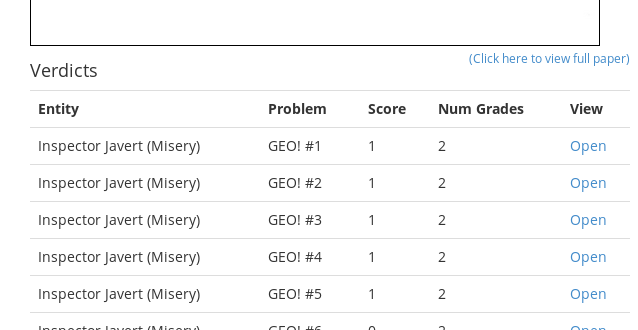
\includegraphics[width=0.6\textwidth]{images/viewpaper2.png}
\end{center}

If the paper has an exam scribble associated,
that will also be displayed,
along with a form to change the name associated to it
(in case of error).

\begin{center}
	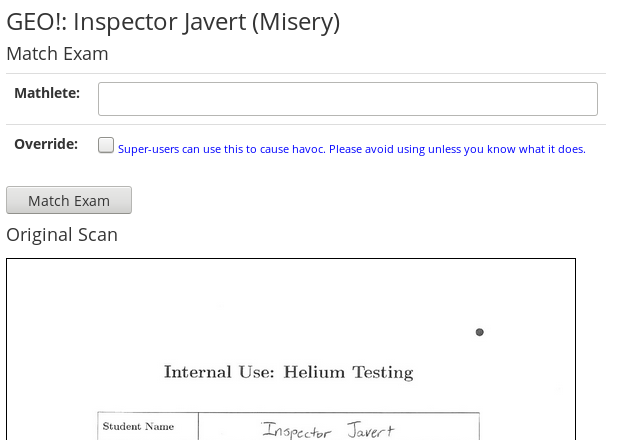
\includegraphics[width=0.6\textwidth]{images/viewpaper1.png}
\end{center}

\section{Troublesome scans}
Scans get marked for administrator attention either by graders,
or by Helium itself when users try to match papers.

There are two ways to get to a list of such papers.
\begin{itemize}
	\ii The ``Find Paper'' link mentioned in previous section. (Recommended.)
	\ii If you open the interface for matching exams for $X$,
	at the very bottom of the page there is a link
	to view only the scans which need administrative attention.
	(Not recommended.)
\end{itemize}
Helium refuses to give out papers to graders
that have been marked with attention until after they have been dealt with.
Here is how you can deal with them.

\subsection{Papers wrong in name only}
There are two types of such errors:
those entered by humans, and those by Helium.

First, sometimes a human will flag a scan for attention
because they can't match it to a student or team
(e.g.\ ``this paper doesn't have a name visible'').
In that case, all you have to do is match it the correct student,
submit that, and then all will be well again.

The tricky situation is auto-marked papers
which occur when a student/team is repeated.
Consider the following situation:
\begin{quote}
	You match a geometry exam to a student ``Christine Daae''.  
	Later on, you try to match another geometry exam
	to the same student ``Christine Daae''.
\end{quote}
This is obviously not okay, and the system will complain.
An error will appear linking to the first \emph{verdict}
it finds for a geometry problem taken by Christine Daae.

\begin{center}
	%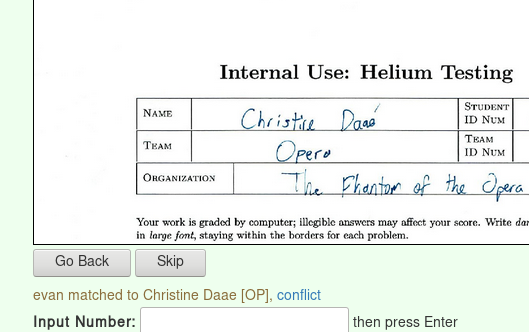
\includegraphics[width=0.7\textwidth]{images/conflict3.png}
	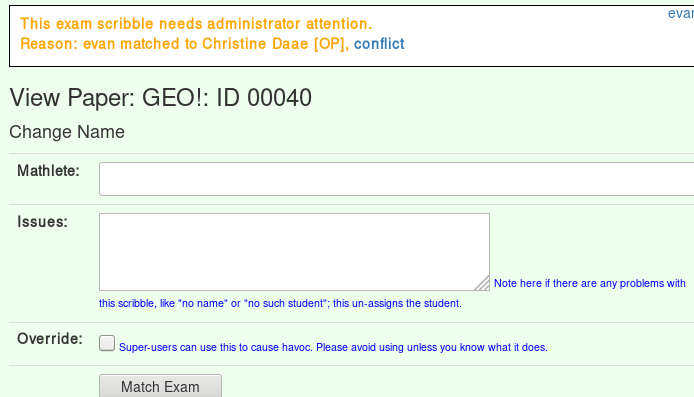
\includegraphics[width=0.7\textwidth]{images/conflict2.png}
\end{center}

At this point you need to fix the error.
There are a couple things you could do.
\begin{itemize}
	\ii If you made the mistake this time,
	then just re-submit the form with the correct name. Easy.

	\ii If you made the mistake the \emph{first} time around,
	then you need to go back and fix it.

	You can do this by clicking on the verdict provided by the system,
	and then opening the exam scribble for that verdict.
	Alternatively, the ``Find Papers'' interface will let you find
	the previous paper as well.
	This will bring you to a match form where you can change the
	name to the correct one.

	\ii As a last resort,
	the ``Override'' switch in the ``full scan'' page (visible only to super-users)
	will forcibly assign the paper,
	and retroactively delete all verdicts and
	problems scribbles to the contrary.
	This is a Bad Idea\texttrademark\ and you should only do it
	if you really understand Helium well and have a compelling reason to do so.
\end{itemize}

\subsection{Other troublesome scans}
\label{sec:trouble_scan}
Graders may also flag scans for administrator attention for other 
more serious reasons:
the scan is upside down, or mis-aligned, et cetera.
This is more serious, since even after you find the name to match it too,
the short-answer graders will be confused by the scan anyways.

To resolve these you should use the following procedure:
\begin{enumerate}
	\ii Match the paper to the correct name at the top of the form,
	but \emph{also} fill in the field with ``Issues''.
	This will both match the paper to a student/team,
	yet still fill in the reason field
	(so Helium will not give the scan to short-answer graders).

	\ii Enter the scores for the paper manually,
	under the ``Change Scores (Admin)'' heading.
	Do this in God mode,
	since you don't want regular graders to have to deal with this.
	
	\ii Release the paper from attention now,
	by re-doing the match in Step 1.
\end{enumerate}

\section{Management}
Several commands are available in the \texttt{manage.py}.
Many of them are revealed through the Helium interface too:
on the dashboard, several links to Helium tasks are available.

When you push one of these such links, you'll be directed to page
which will auto-refresh once the task is done.
This is necessary since the task can potentially take very long
(algorithmic scoring).
\begin{center}
	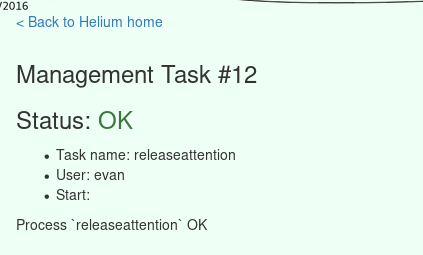
\includegraphics[width=0.7\textwidth]{images/viewtask.png}
\end{center}

We'll talk more about these commands in the next chapter.

\section{Other Administration}
The Django admin interface can be used if there
is some operation you need to do not supported by the existing views.

\subsection{Someone uploaded PDF to wrong exam!}
Well, that's a bummer.
Delete the relevant PDF file from the Django admin interface.
This will kill off the exam scribbles and problem scribbles too.

As of December 2016, deleted problem scribbles will also kill
off the verdict to which they were attached.
That should mostly save things. No promises though.

\subsection{A page is rotated!}
See Section \ref{sec:trouble_scan}.

\subsection{A problem had the wrong answer!}
Well, guess you need to re-grade said problem.

If you open the ``Verdicts'' admin,
under the ``Action'' menu near tho top,
there is a command called ``reset verdict''.
If you select a bunch of verdicts and use this command,
all the evidence's associated to that verdict will be erased.

In particular, if you have an entire problem that needs to be regraded,
then you should use the panel on the right to filter
only the verdicts for that particular problem,
and then use this command in order to reset them all.
